\documentclass[man, floatsintext]{apa6}
% floatsintext so that figures show up where we want them to (https://www.tug.org/pracjourn/2012-1/beitzel/beitzel.pdf) 
\usepackage{lipsum}
\usepackage{amsmath}

\usepackage[american]{babel}
\usepackage{ulem}
\usepackage{graphicx} 
\usepackage{csquotes}
\usepackage{hyperref}
\usepackage[style=apa,sortcites=true,sorting=nyt,backend=biber]{biblatex}
\DeclareLanguageMapping{american}{american-apa}
\addbibresource{project1.bib}

\title{Analysis of Customer Churn at Telco}

\shorttitle{Customer Churn}

\author{Pedro Uria, Sean Pili, and Zachary Buckley}

\affiliation{George Washington University}

\abstract{
  TODO: This is the abstract.
}

\begin{document}
\maketitle

\section{Introduction and Background Research}
\paragraph{Churn Rate}

In business, churn rate is the percentage of a company's customers that terminate their relationship with that company \textbf{during a given time period}. In the telecommunications industry, churn rates can be especially high because there is fierce competition and the market is saturated. In fact, in their (\textbf{who is they}?) study of factors that explain customer churn rates for an Indian telecommunications company \textbf{by the name of} Asamoah et. al, \textbf{they} mention that ``worldwide, the rate of customer churn in the telecom service industry ranges from 20 percent to 40 percent per year'' (224) \textbf{I guess you want to insert a reference here?}. If a company loses 20-40 percent of its existing customer base every year, that can have a significant \textbf{and} negative \sout{on} effect on its revenue, regardless \textbf{of} how many new customers they obtain.  Consequently, many companies in saturated markets keep track of monthly, quarterly \textbf{and/}or yearly churn rates in an attempt to identify defining characteristics of customers who churn, in order to predict and eventually reduce their customer churn rate. 

Much of the scientific research on reducing customer churn across all industry verticals involves using logistic regression or \textbf{other} classification methods to predict which customers will churn in a given \textbf{time} period (typically monthly.) Common features used \sout{to classify which customers will churn across different industry verticals} \textbf{as classifiers} include different aspects of customer purchasing behavior, their tenure (the length of a customer's relationship with a company), their account charges,  and frequency of their transactions (depending on the type of business). In 2015, Jarvis et al. ran an analysis on consumer data from an Australian streaming DVD rental service to determine if adding features that measure ``customer satisfaction, attitude and commitment'' to models meant to classify whether or not a customer will churn would increase their prediction accuracy.  Interestingly, Jarvis et. al. found that ``the most significant predictor of churn in [customer purchasing habits, satisfaction and attitude] was a measure of uncertainty and commitment: the number of times a customer changed their subscription plan''. Jarvis et. al did not explain how the customers changed their plans, (i.e. did the customers add or subtract services from their plans or alter other aspects of their plans entirely?)  Additionally

\hspace{0.5mm}

\paragraph{Telco Dataset}

The Telco Customer Churn Dataset we will be using throughout this paper contains information about the customers from an unidentified telecommunications company. The data was uploaded to \href{https://www.kaggle.com/blastchar/telco-customer-churn}{Kaggle} by a user named blastchar. \cite{blastchar_2018} ??? The dataset originates from a sample dataset provided by IBM for exploring the capabilities of IBM's Watson Analytics services. IBM uses the data in a walkthrough of building a model for predicting whether a customer will leave the company, with the explicit goal of creating better customer retention programs. \cite{ibm_telco_2015} There are a number of sample data sets provided by IBM for similar walkthroughs related to their Watson Analytics system. \cite{ibm_data_2015} We were unable to determine conclusively if the Telco Dataset we are interested in for this paper was based on data from a real telecommunications company, or if the data was synthetically generated for the purposes of demonstrating the Watson Analytics system's capabilities.

\section{Research Question and Hypotheses}
\paragraph{Research Question}

Are there significant relationships between the following variables and \texttt{Churn}?
\begin{itemize}
\item{\texttt{Contract Type}}
%\item{Paperless Billing}
%\item{Partner}
%\item{Device Protection}
%\item{Tech Support}
%\item{Online Backup}
\item{\texttt{MonthlyCharges}}
\item{\texttt{Tenure}}
\end{itemize}

???Original Research Question:
Is Churn rate independent of the type of contract a customer holds and if the average tenure of customers who churned is different that the average tenure of customers who are remaining with the company.???

\paragraph{Hypotheses}

\begin{itemize}
\item \texttt{ContractType} $\begin{cases}
H_0: \texttt{Churn} \hspace{1mm} \text{and}  \hspace{1mm} \texttt{ContractType} \hspace{1mm} \text{are independent} \\
H_1: \texttt{Churn} \hspace{1mm} \text{and} \hspace{1mm} \texttt{ContractType} \hspace{1mm} \text{are not independent}
\end{cases}$
\item \texttt{MonthlyCharges} $\begin{cases}
H_0: \mu_{\text{Churn}} = \mu_{\text{NotChurn}} \\
H_1: \mu_{\text{Churn}} \neq \mu_{\text{NotChurn}}
\end{cases}$ 
\item \texttt{Tenure} $\begin{cases}
H_0: \mu_{\text{Churn}} \geq \mu_{\text{NotChurn}} \\
H_1: \mu_{\text{Churn}} < \mu_{\text{NotChurn}}
\end{cases}$ 
\end{itemize}

\textbf{IN THE CASE OF MonthlyCharges, IT DOESN'T SEEM FAIR TO BEGIN WITH A ONE TAILED HYPOTHESIS BECAUSE IT ISN'T SO CLEAR WHAT TO EXPECT, HOWEVER, IN THE CASE OF Tenure IT DOES MAKE SENSE TO EXPECT THE MEAN OF NOT CHURN TO BE GREATER THAN THE MEAN OF CHURN}

%\paragraph{Methods}

%E

\section{EDA and Model Results} 

\paragraph{Contract Type}
\texttt{ContractType} is a categorical value that tells us whether a customer has a monthly, 1-year or 2-year contract. 

\hspace{0.5mm}

\noindent\begin{minipage}{0.54\textwidth}
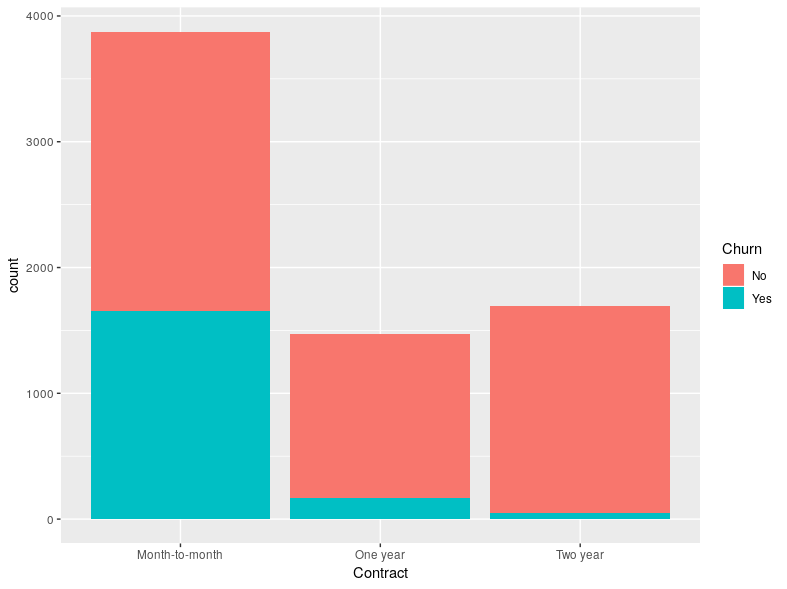
\includegraphics[width = \linewidth, height = 72mm]{CountvsContractTypebyChurn}
\end{minipage}
\hfill
\begin{minipage}{0.42\textwidth} The stacked bar plot to the right gives us a first look at the data. A clear difference in the ratio of people who churn and who don't churn can be seen when comparing the monthly contract with the other two types. By computing the differences on the observed and expected frequencies, we can check if this difference is statistically significant. 
\end{minipage}  

\hspace{0.5mm}

This can be done by running a $\chi^2$-test in R, which returns $\chi^2 = 1184.6$ and $p < 2.2 \cdot 10^{-16}$. Thus we reject the null hypothesis at the $5 \%$ level of significance and say that \texttt{ContractType} and \texttt{Chrun} are related.  

\textbf{TALK ABOUT TENURE HISTOGRAM}

\paragraph{Billing}

In this section we first did \textit{EDA} on \texttt{MonthlyCharges}, a continuous variable that gives the amount of dollars charged to a customer each month (thus, in this case we shall not use a $\chi^2$-test, which only makes sense for categorical data). The goal was to have a first look at how this variable behaved for customers who churned and for customers who did not churn, in order to asses which statistical test to use to check our alternate hypothesis. 

%\hspace{0.5mm}

\noindent\begin{minipage}{0.54\textwidth}
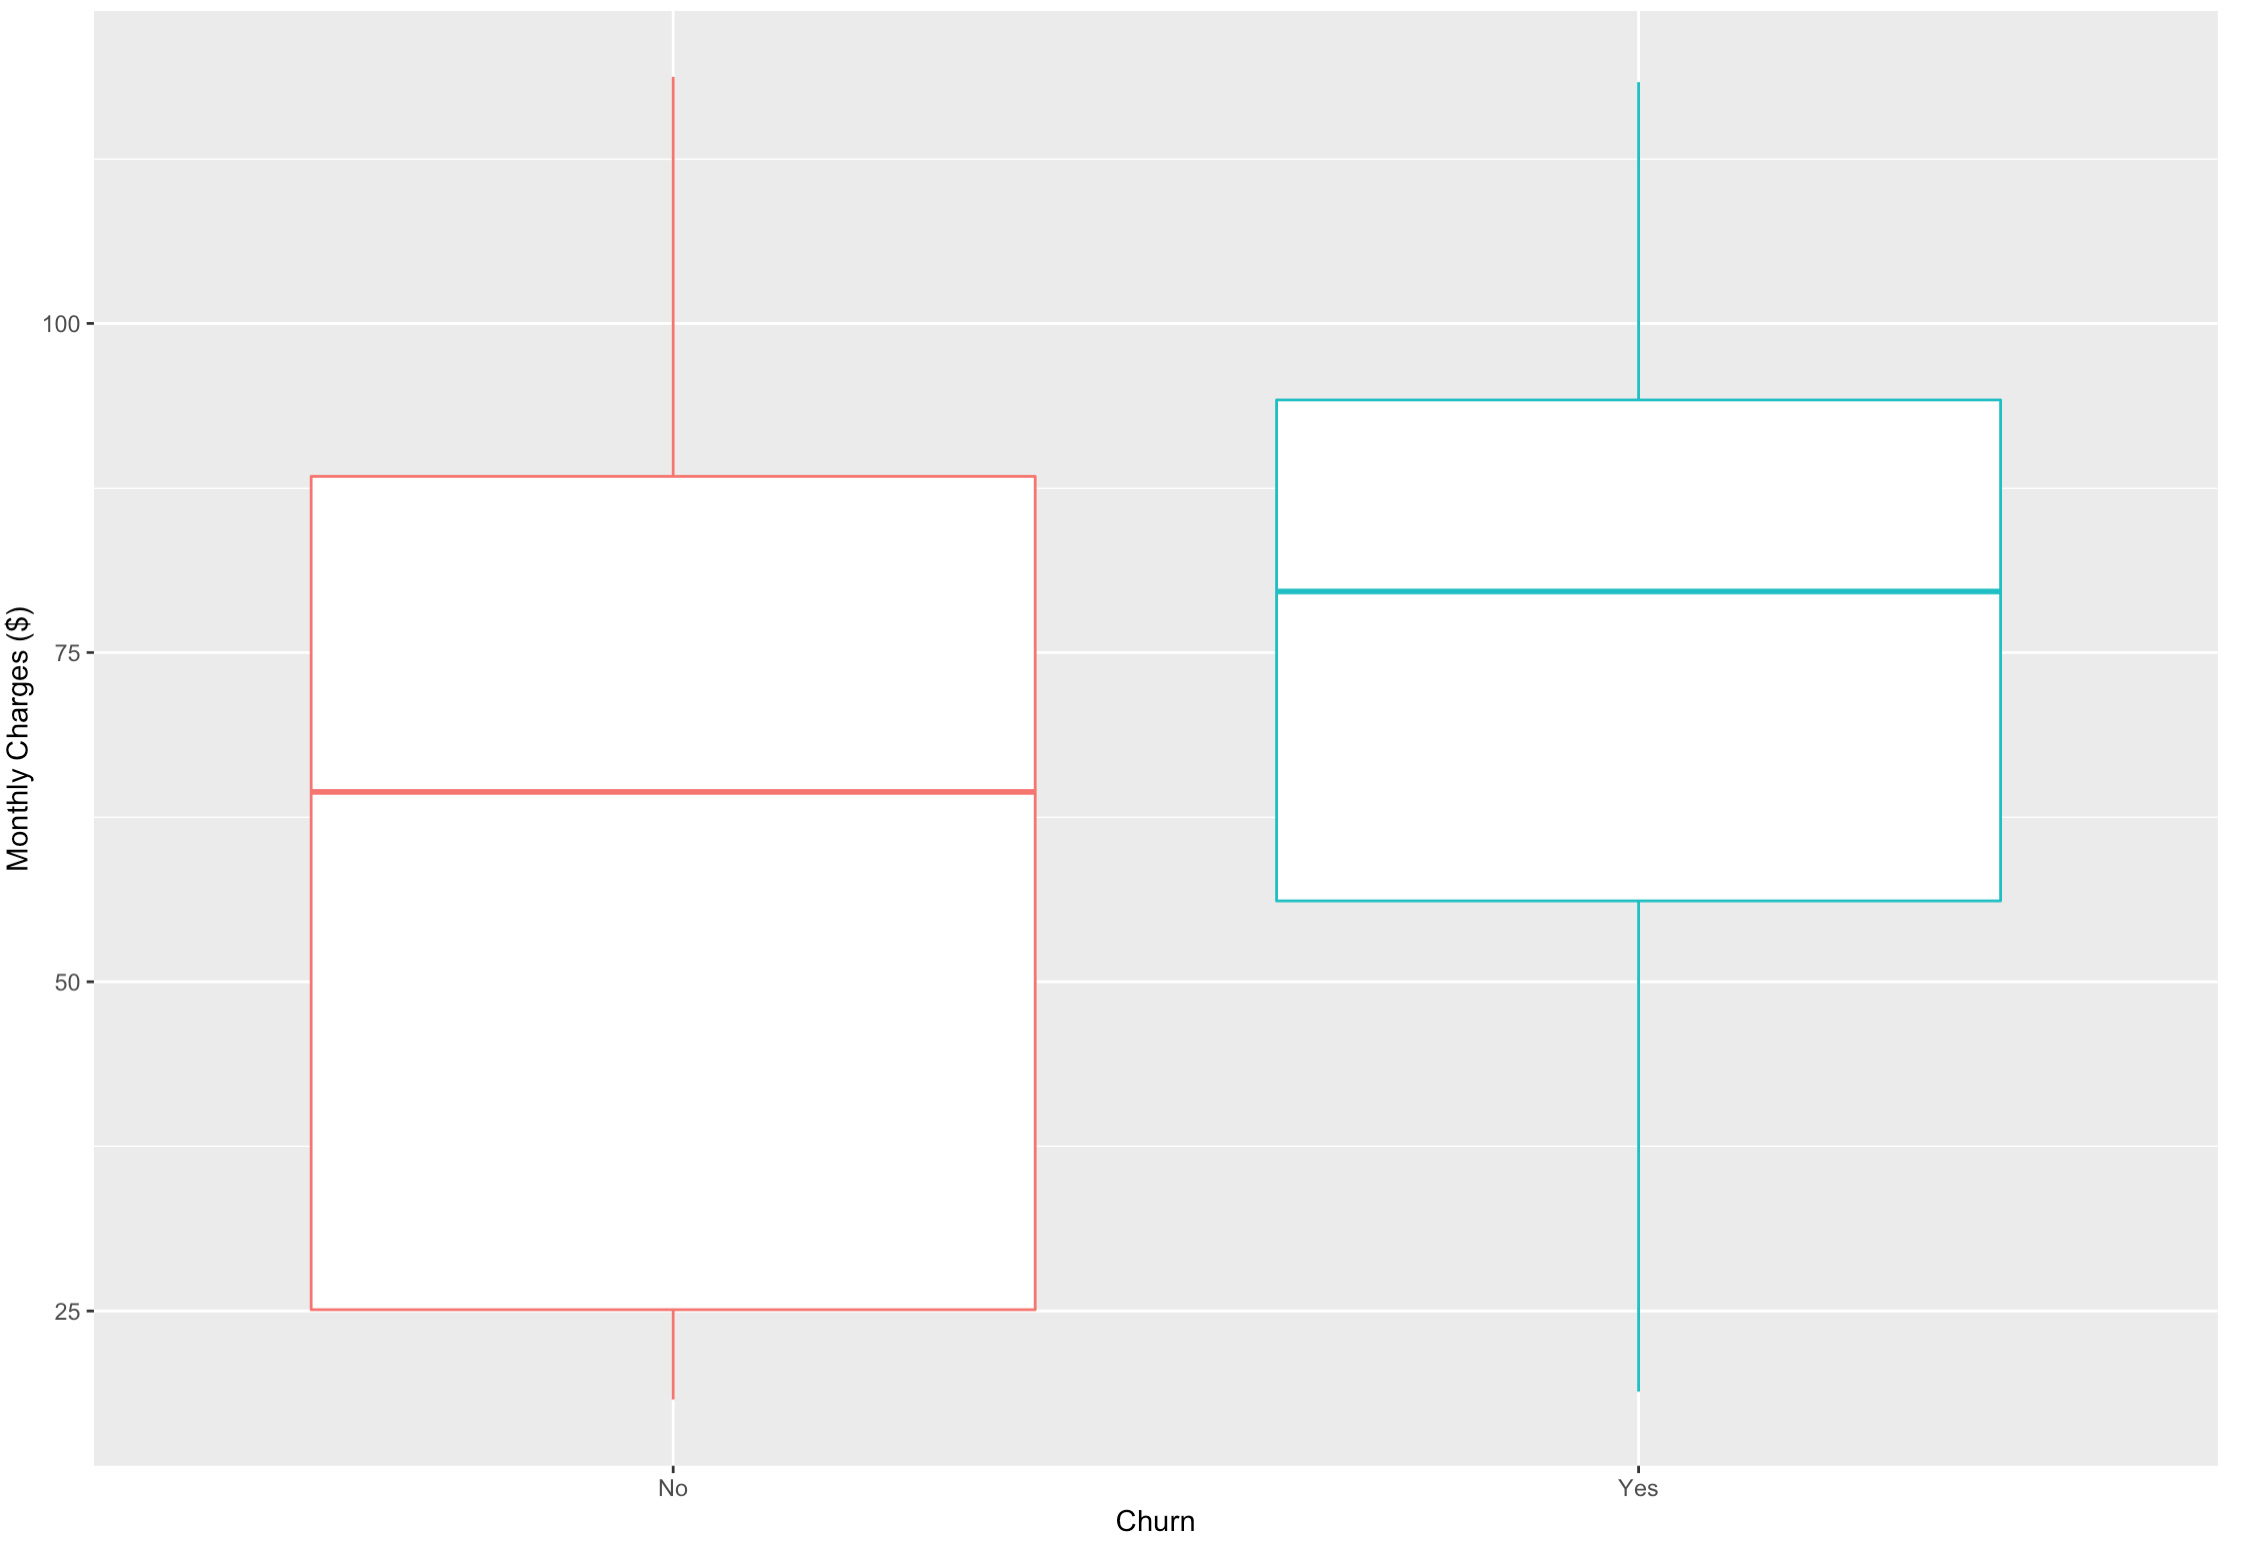
\includegraphics[width = \linewidth, height = 64mm]{boxplot_MonthlyChargesvsChurn}
\end{minipage}
\hfill
\begin{minipage}{0.43\textwidth} On the left there is a boxplot for \texttt{MonthlyCharges}, grouped by \texttt{Churn}. We can see how the variances are clearly different, and because of this we can't use a Student's $t$-test to tell whether $\mu_{\text{Churn}} = \mu_{\text{NotChurn}}$ or not. Instead, we will use a Welch's $t$-test, which does not assume equality of variances. 
\end{minipage}


\noindent\begin{minipage}{0.54\textwidth}
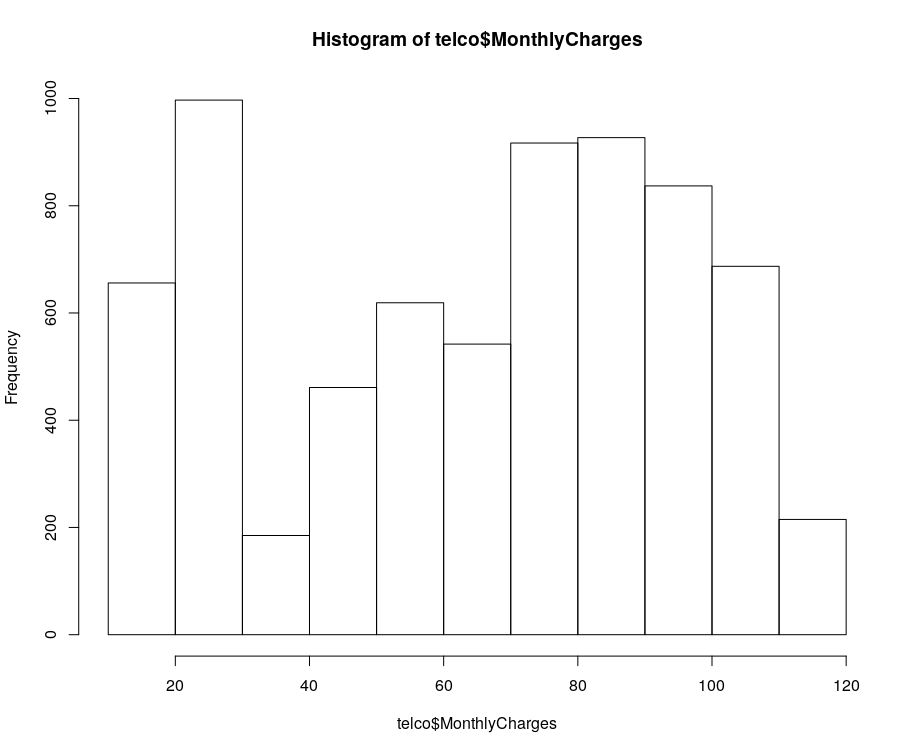
\includegraphics[width = \linewidth, height = 72mm]{hist_MonthlyCharges}
\end{minipage}
\hfill
\begin{minipage}{0.43\textwidth} Notice how the distribution of the monthly charges is not normally shaped. However, what we are comparing are means, and the Central Limit Theorem assures us that these means will follow a normal distribution for a large enough sample size (our case), which enables us to perform the Welch's $t$-test. 
\end{minipage}

\hspace{0.5mm}

By looking at the boxplot we also realize that the mean of monthly charges for customers who churned appears to be greater than that of the customers who have not churned. Thus, we modify our original hypothesis to $H_0: \mu_{\text{Churn}} \leq \mu_{\text{NotChurn}}$ and $H_1: \mu_{\text{Churn}} > \mu_{\text{NotChurn}}$. Upon running this test (one-tailed) on R, we get a $p$-value $< 2.2 \cdot 10^{-16}$, so we reject $H_0$ and say that the data is statistically significant  at the $\alpha = 0.05$ level to conclude that customers who churned are paying more on average that customers who have not churned,
\paragraph{Tenure}

The process for \texttt{Tenure} was analogous to the one for \texttt{MonthlyCharges}, as this continuous variable presented similar differences in variance and is also non-normally shaped. 

\hspace{0.5mm}

\noindent\begin{minipage}{0.485\textwidth}
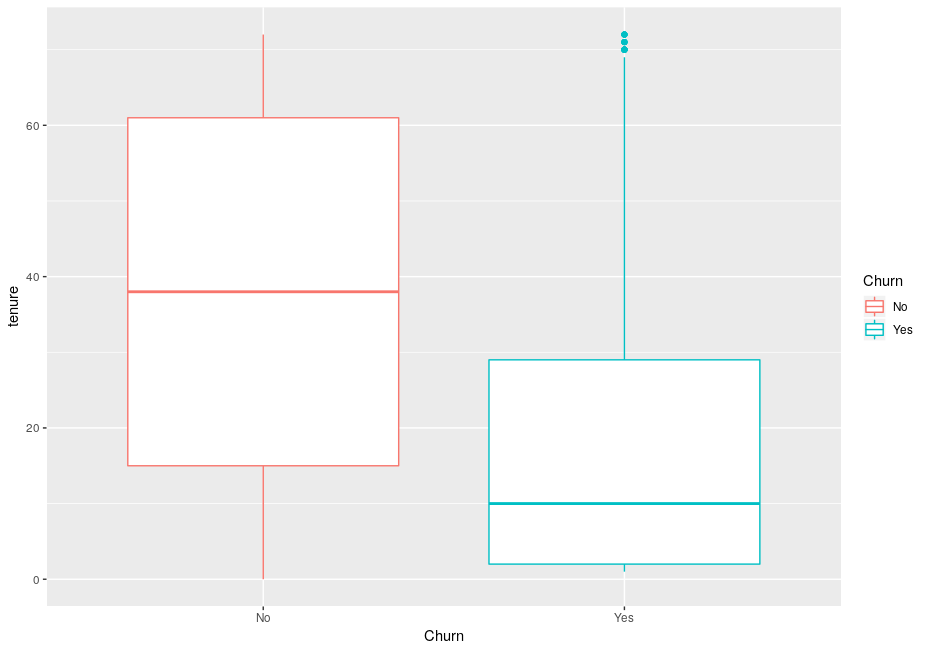
\includegraphics[width = \linewidth]{boxplot_tenurebyChurn}
\end{minipage}
\hfill
\begin{minipage}{0.5\textwidth} 
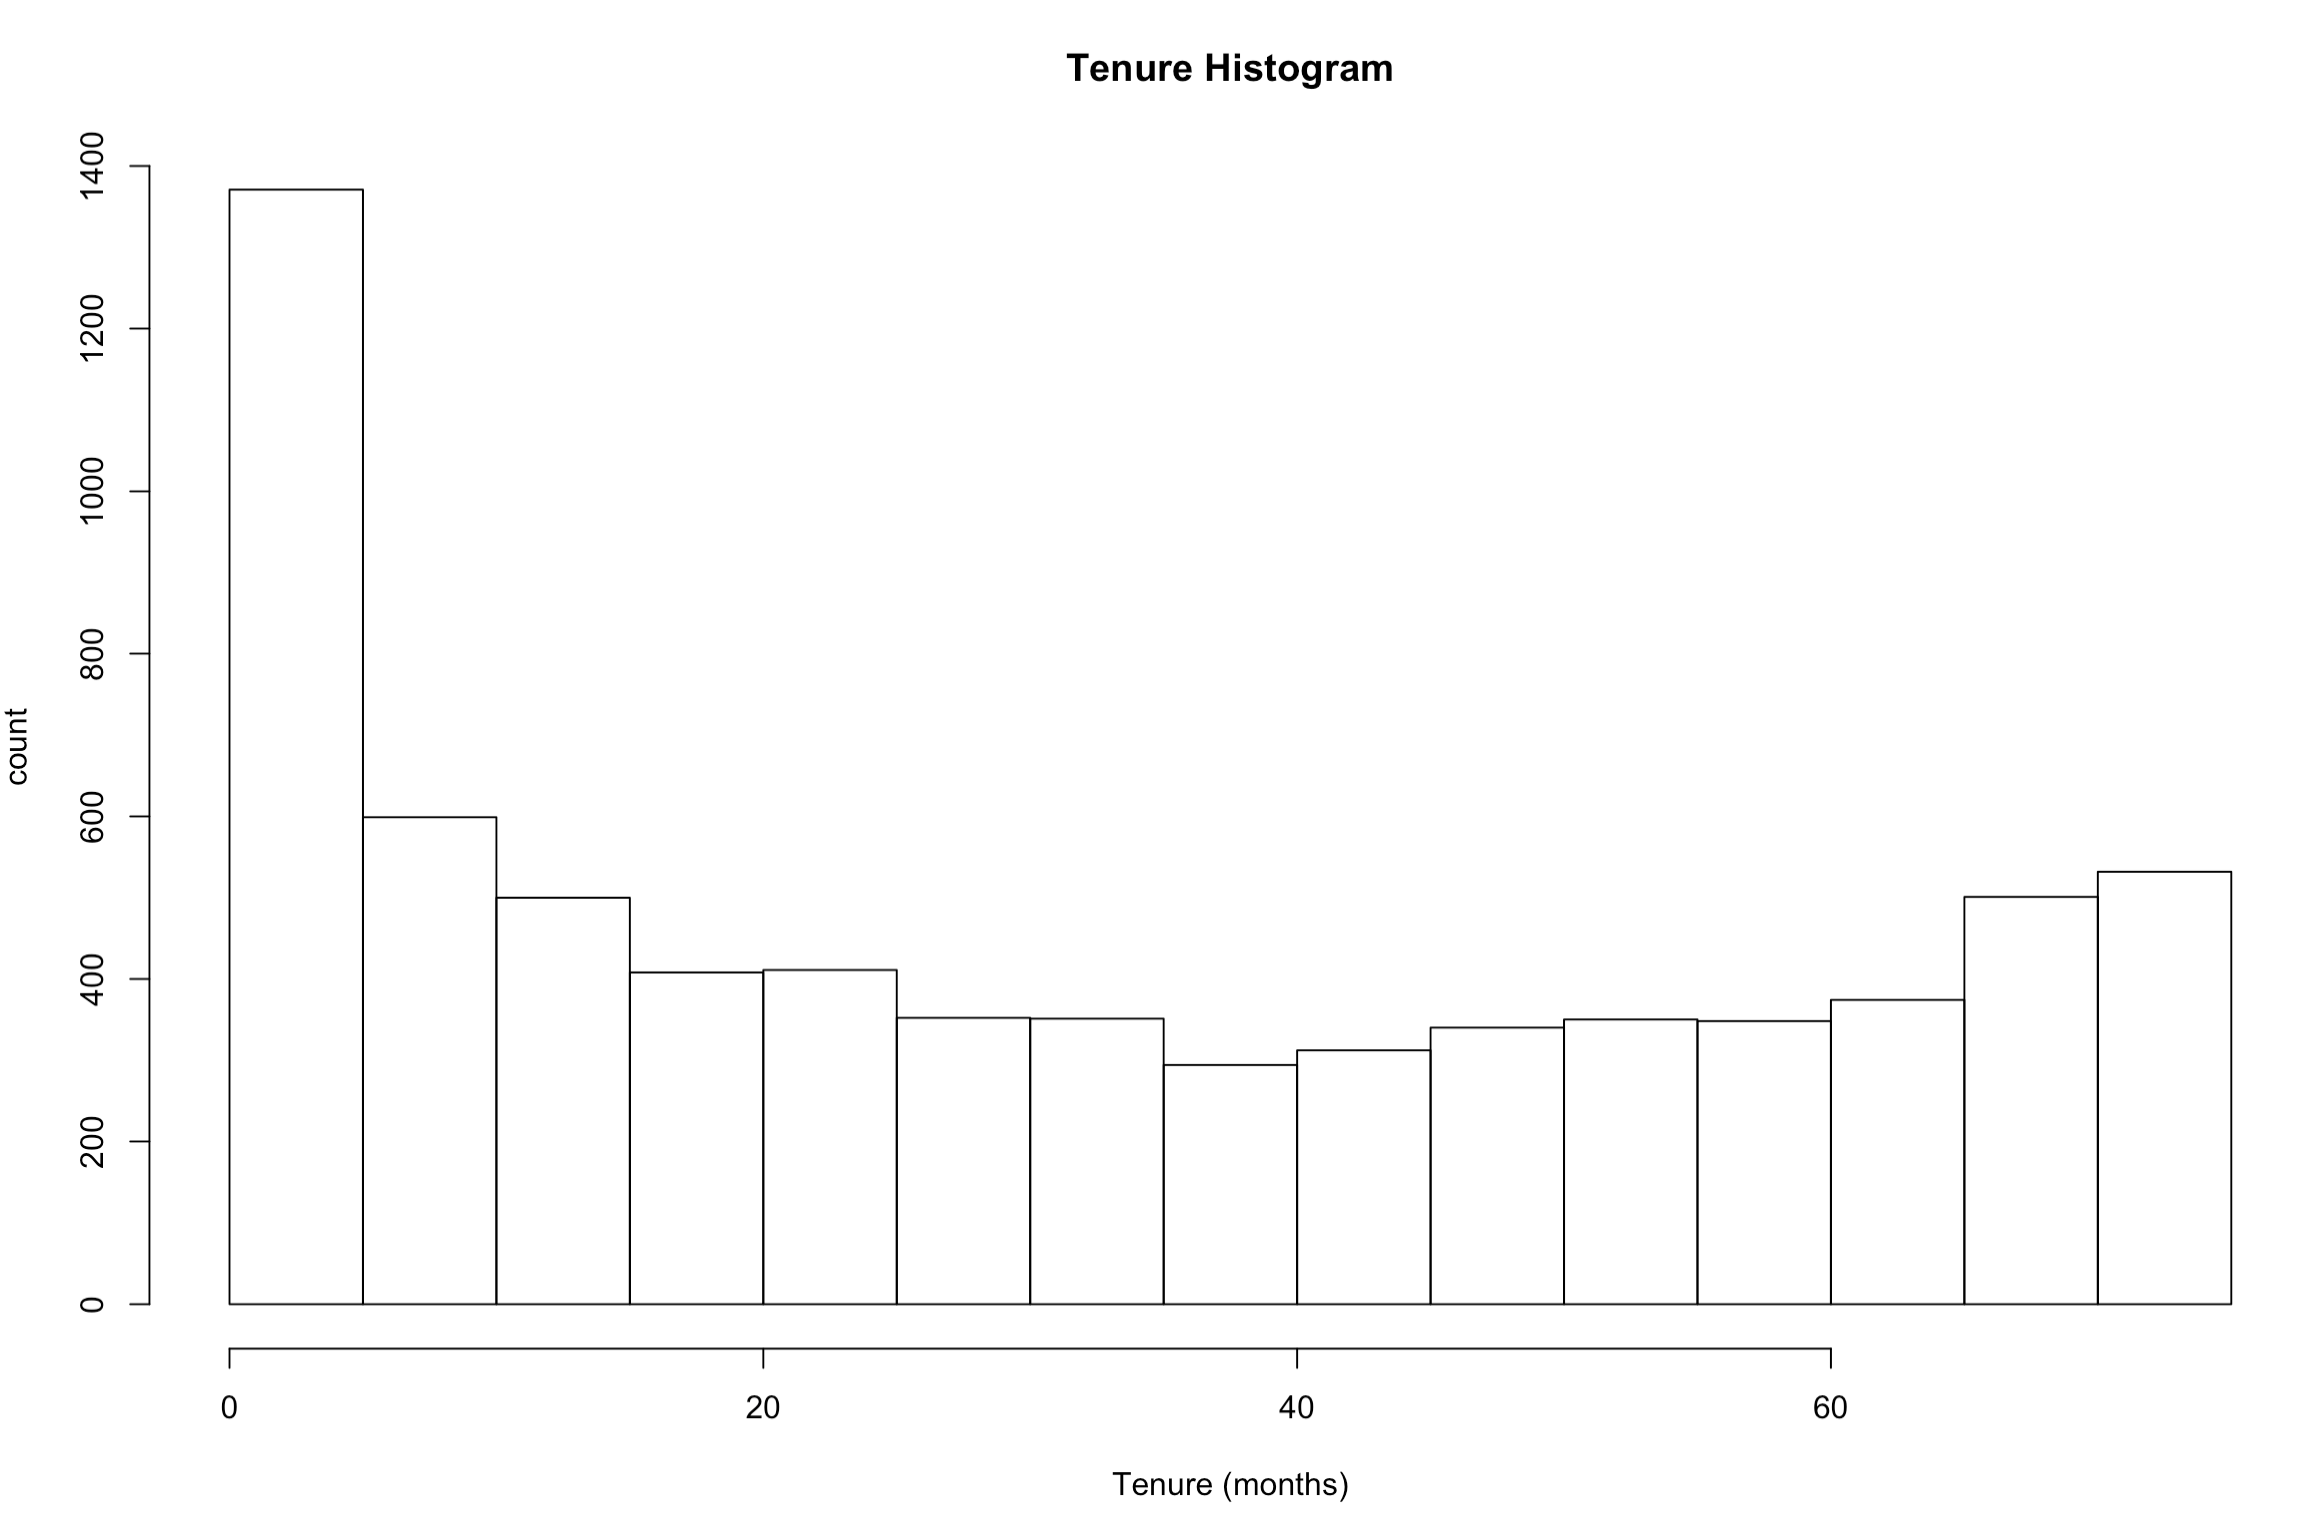
\includegraphics[width = \linewidth]{histogram_Tenure}
\end{minipage}

\hspace{0.5mm}

In this case, we also get a very small $p$-value (again $< 2.2 \cdot 10^{-16}$), so we reject the null hypothesis that  $H_0: \mu_{\text{Churn}} \geq \mu{X}_{\text{NotChurn}}$ and say that at the $5 \%$ significance level, customers who haven't churned have been longer on average with the company. 


\section{Conclusions}

By performing a combination of Explanatory Data Analysis and Hypothesis Testing, we have come to the conclusion that, as we expected, there are significant relationships between \texttt{Churn} and the three variables \texttt{ContractType}, \texttt{MonthlyCharges} and \texttt{Tenure}. 

In particular, the dependence between \texttt{ContractType} and \texttt{Churn} has been tested by a $\chi^2$-test. People who have a monthly contract are the most likely to churn, as common sense would indicate. We have also seen, by running one-tailed $t$-tests, that the mean of \texttt{MonthlyCharges} is greater for customers who churned, and that the mean of \texttt{Tenure} is greater for customers who haven't churned. 

\textbf{I GUESS WE SHOULD SAY SOMETHING ABOUT THE RESEARCHERS FINDINGS HERE TOO}

\appendix
\section{Best Variables for Linear Regression?}
\newpage
\printbibliography
\end{document}
